\documentclass%
  [/Users/rodrigo/Documents/TUe/thesis/latex/topic/fluctuation_strength/
  literature_review.tex]
  {subfiles}

\begin{document}

\section{Psychoacoustics: Facts and models}

This book contains a chapter dedicated to discuss fluctuation strength and its
properties. First, several variables and their interactions with fluctuation
strength will be described; then, a model for fluctuation strength will be
presented.

\subsection{Fluctuation Strength}

Fluctuation strength corresponds to the sensation that arises when a sound
presents a slow envelope (i.e., a modulation signal whose frequency is less than
20 Hz). Fluctuation strength is closely related to roughness, the difference
between the two being the frequency of the envelope.
Fluctuation strength can have a significant effect on the pleasantness of sound,
and a particularly clear example of this are alarms, which must have a sharp and
distinctive sound.

The effect of fluctuation strength can be seen as a temporary masking pattern on
the original signal, in which the modulation depth is of utmost importance. This
is also the case for roughness, which resembles fluctuation strength in this
regard.

\subsection{Dependencies of Fluctuation Strength}

As a reference, the unit of 1 vacil is defined as a 1 kHz tone sound having a
SPL of 60 dB, with an amplitude-modulated envelope of 4 Hz and a modulation
index of 1. The maximum of this quantity seems to occur around 4 Hz, regardless
of the modulation technique used (\cref{fig:flucstrenvmodfreq}).

\begin{figure}
  \centering
  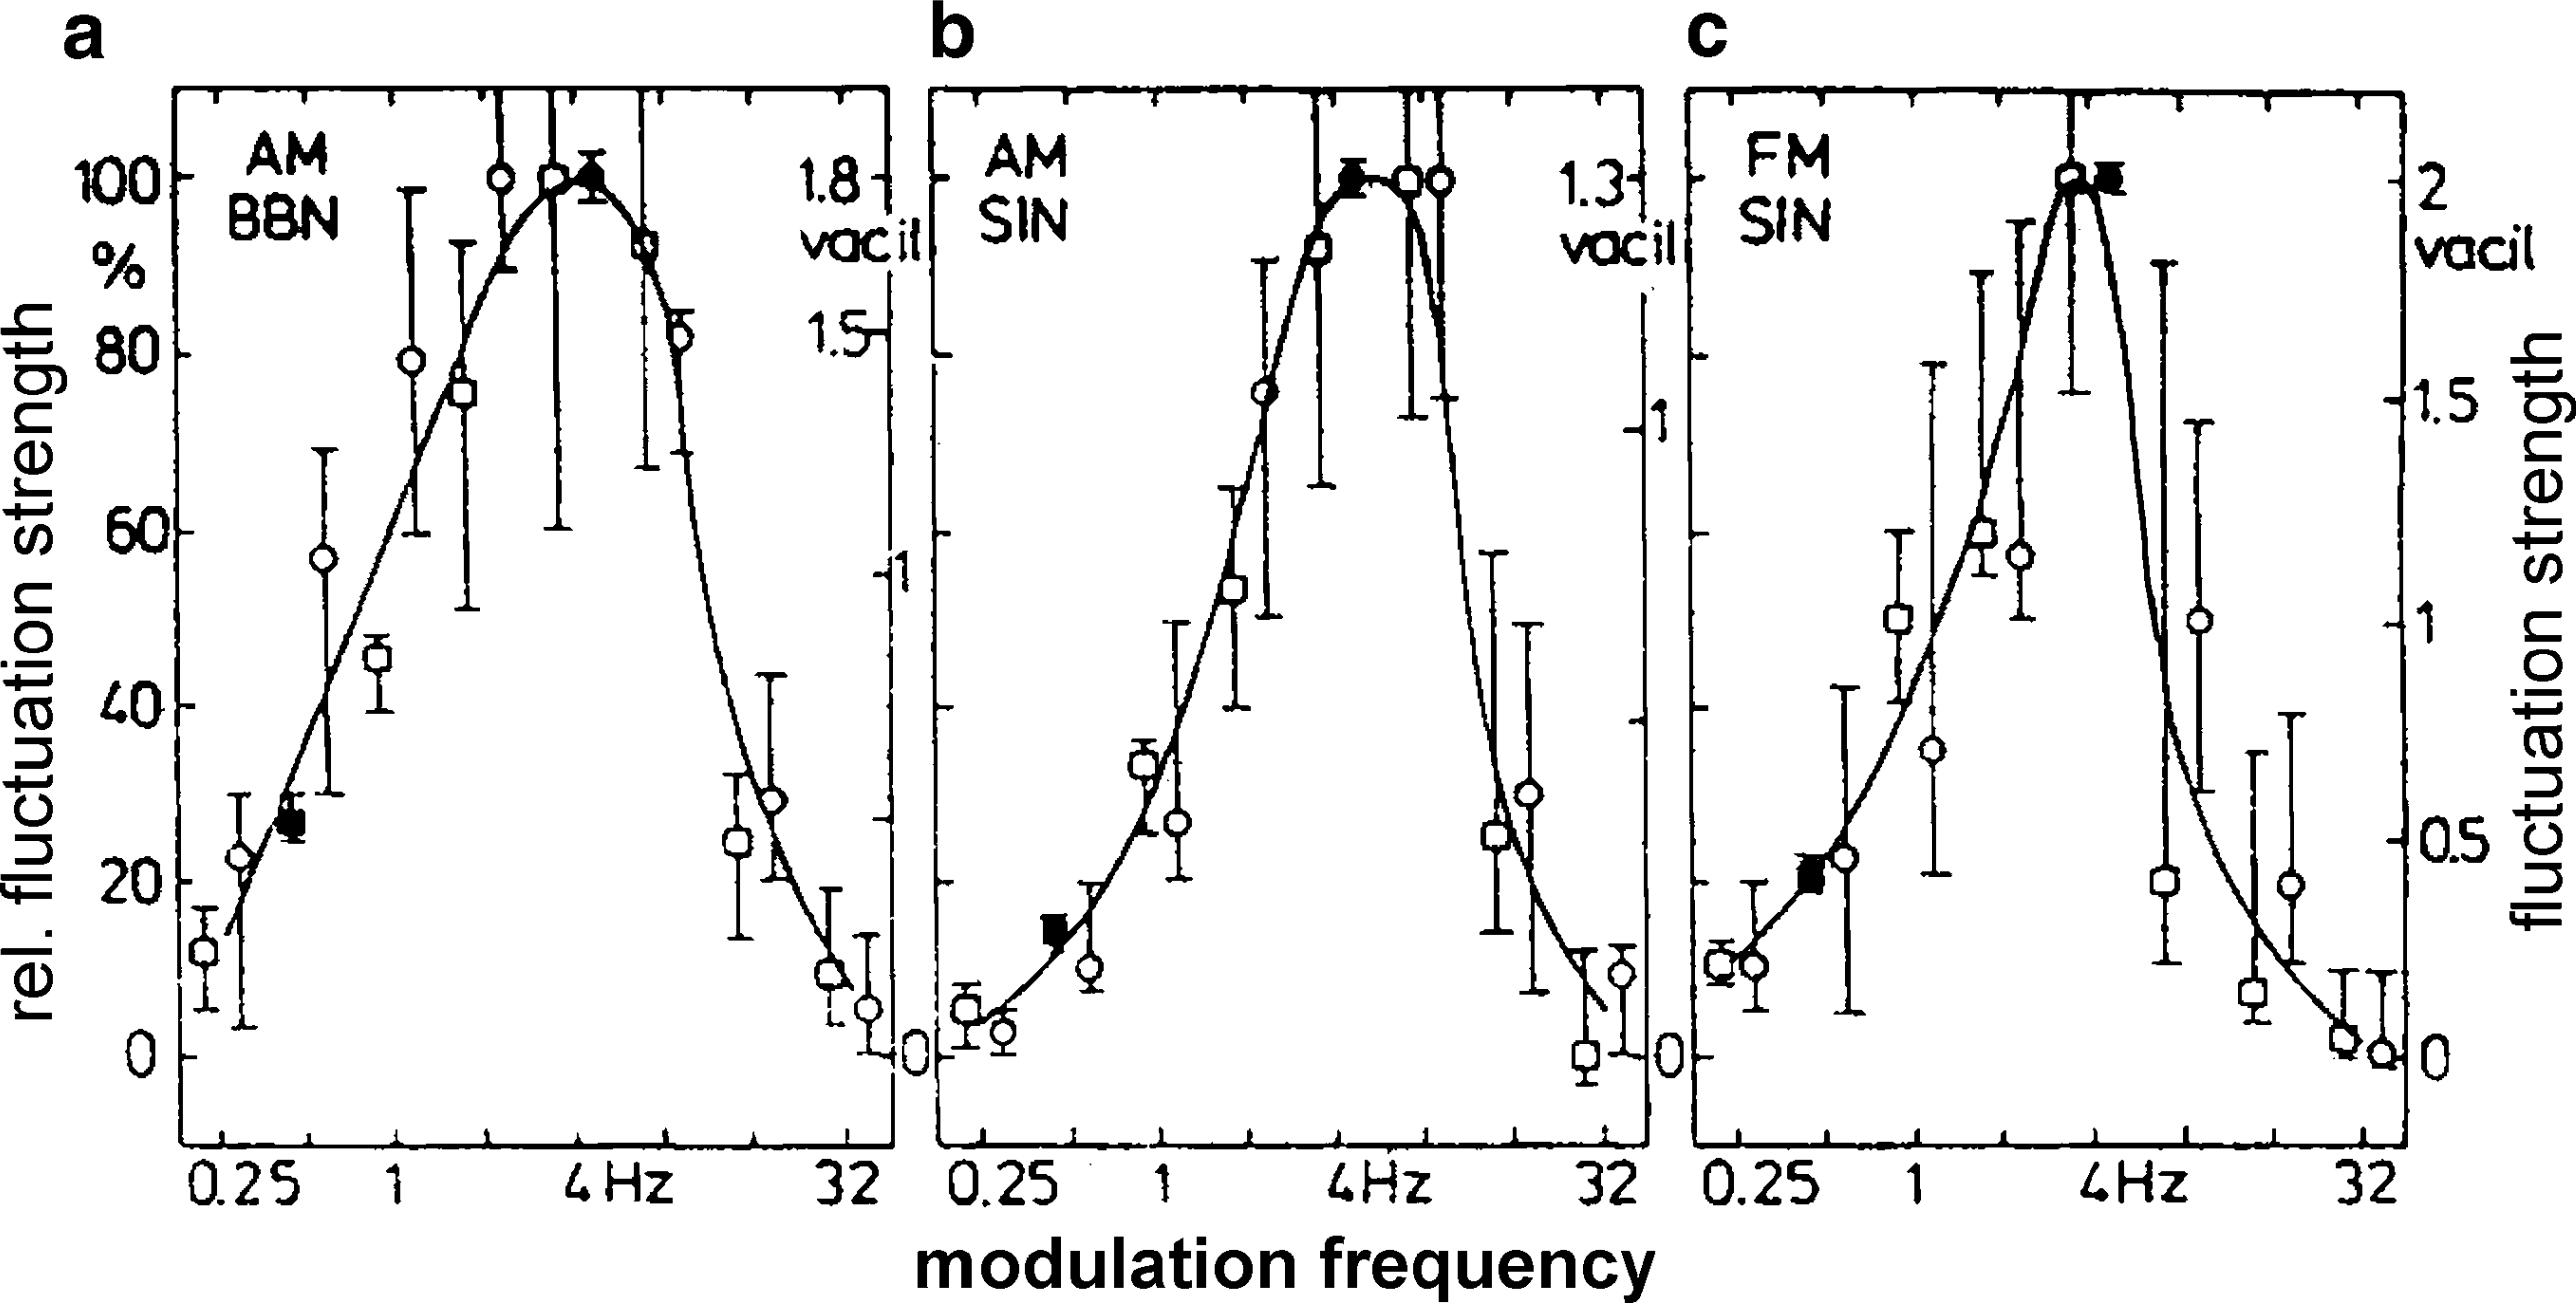
\includegraphics[height=5cm]{FluctuationStrengthVsModulationFrequency}
  \caption{Fluctuation strength as a function of modulation frequency for (a)
    amplitude-modulated broad-band noises, (b) amplitude-modulated tones and (c)
    frequency-modulated tones~\cite[pp.~248]{Fastl2007Psychoacoustics}}
\label{fig:flucstrenvmodfreq}
\end{figure}

It seems that a relation between fluctuation strength and speech production
exists, as the normal production rate of syllables during normal conversation
speed is about 4 syllables/second. This coincides with the frequency in which a
maximum value of fluctuation strength occurs (4 Hz).

Regarding sound pressure level (SPL) and fluctuation strength,
\cref{fig:flucstrenvsndpreslvl} shows their relation for two different stimuli
(tones and broad-band noise) and two modulation techniques (amplitude modulation
and frequency modulation). An increase in SPL entails an increase of fluctuation
strength, this being stronger when using amplitude-modulation.

\begin{figure}
  \centering
  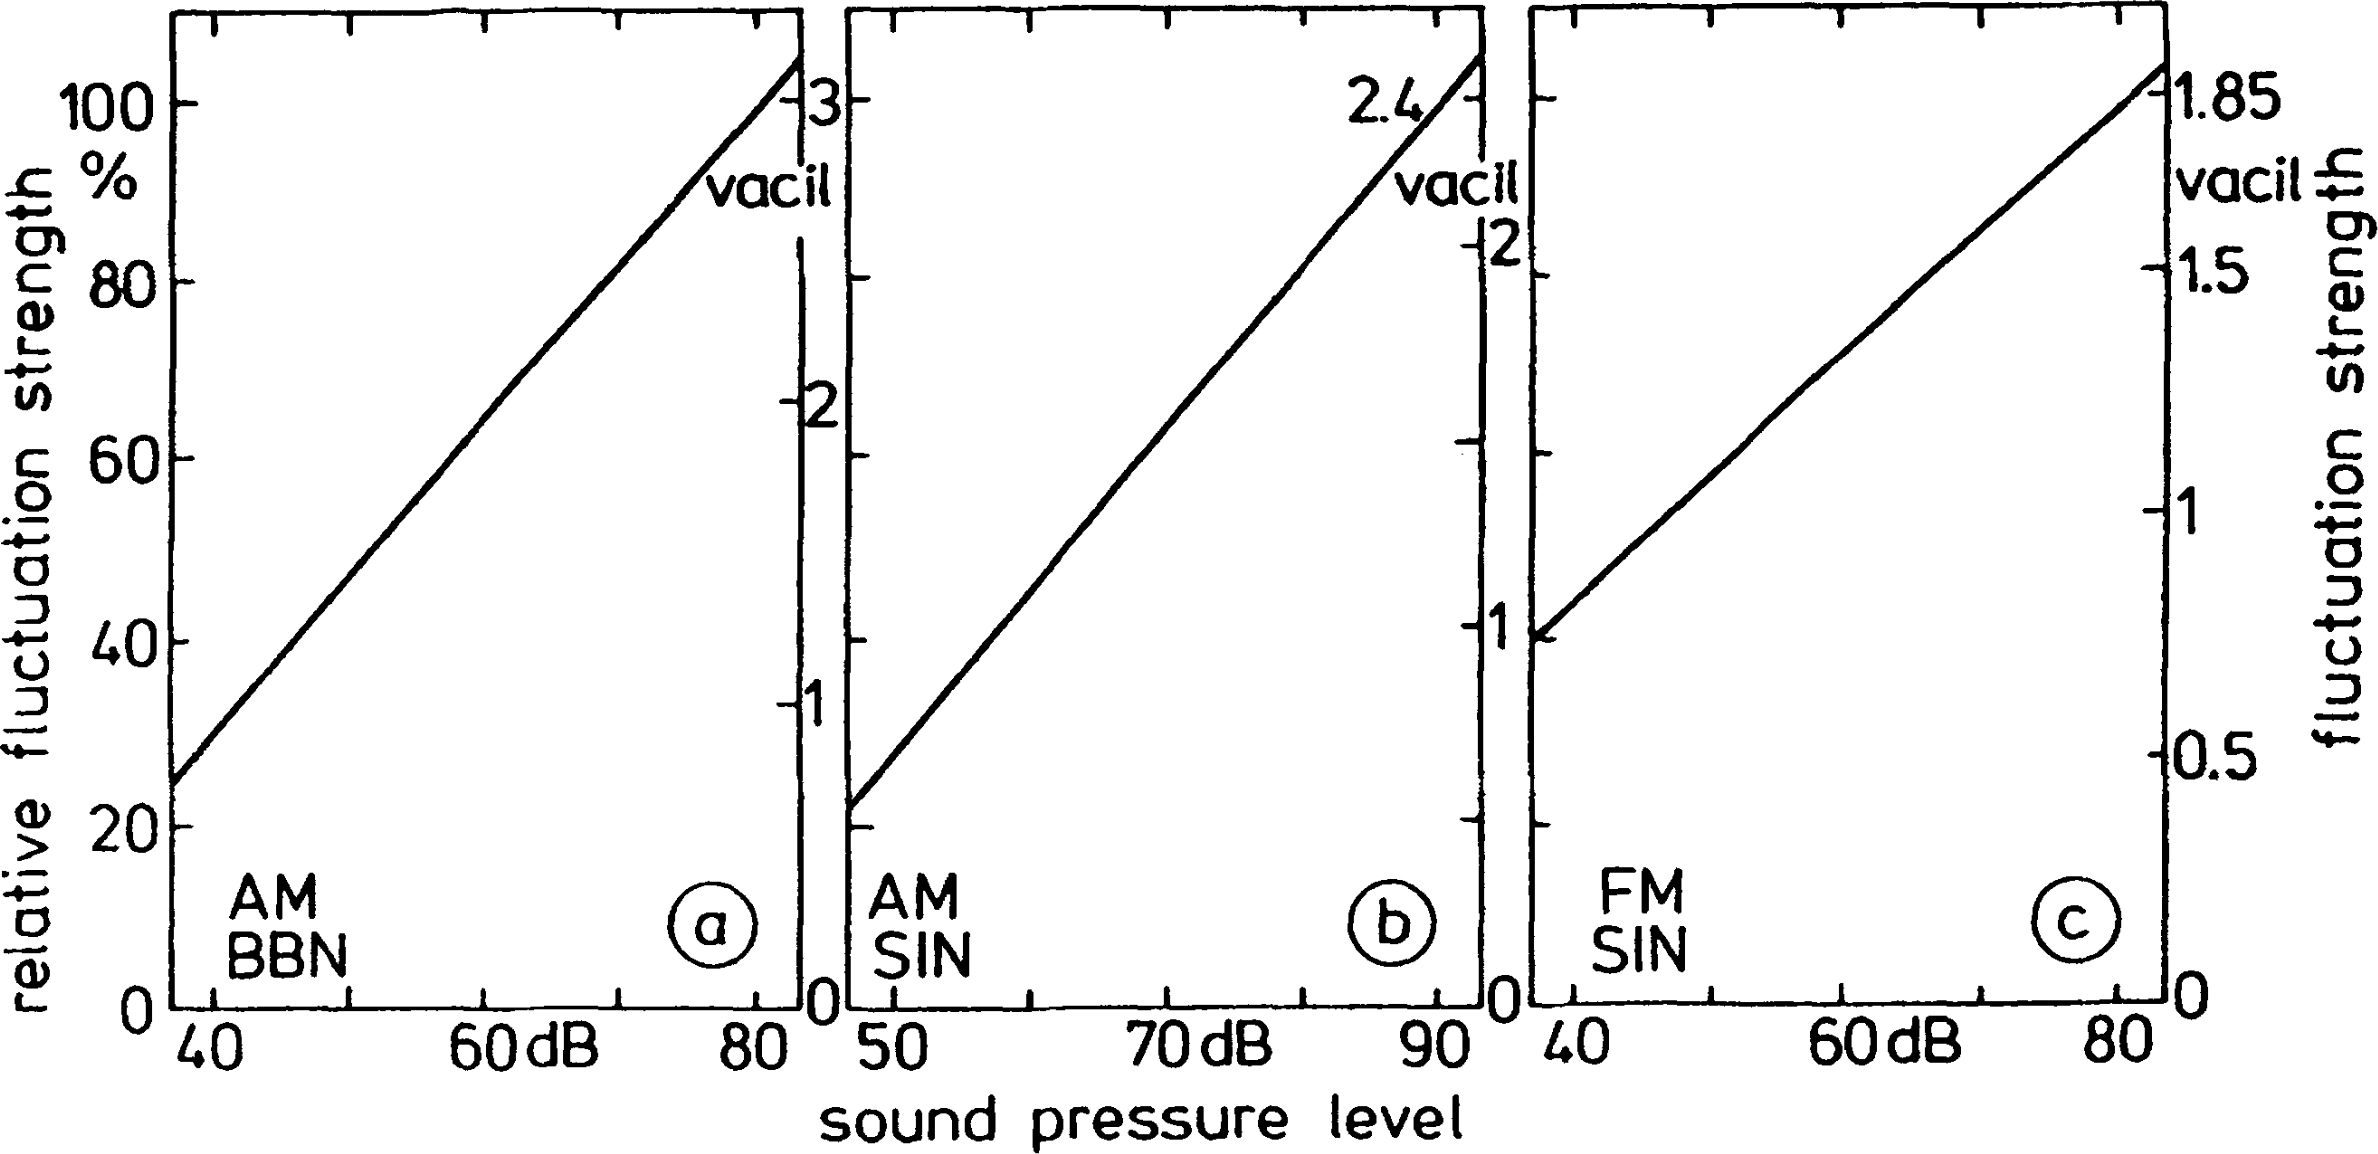
\includegraphics[height=5cm]{FluctuationStrengthVsSoundPressureLevel}
  \caption{Fluctuation strength as a function of sound pressure level for (a)
    amplitude-modulated broad-band noises, (b) amplitude-modulated tones and (c)
    frequency-modulated tones; modulation frequency of
    4Hz~\cite[pp.~249]{Fastl2007Psychoacoustics}}
\label{fig:flucstrenvsndpreslvl}
\end{figure}

Next the effect of modulation depth on fluctuation strength is analyzed, which
can be observed on \cref{fig:flucstrenvsmoddep}. It can be observer than,
between 3 dB and 30 dB the relation between fluctuation strength and modulation
depth is somewhat linear. After reaching a maximum value at around 30 dB, which
corresponds to a modulation factor of 94\%, fluctuation strength remains
constant with further increments of modulation depth.

\begin{figure}
  \centering
  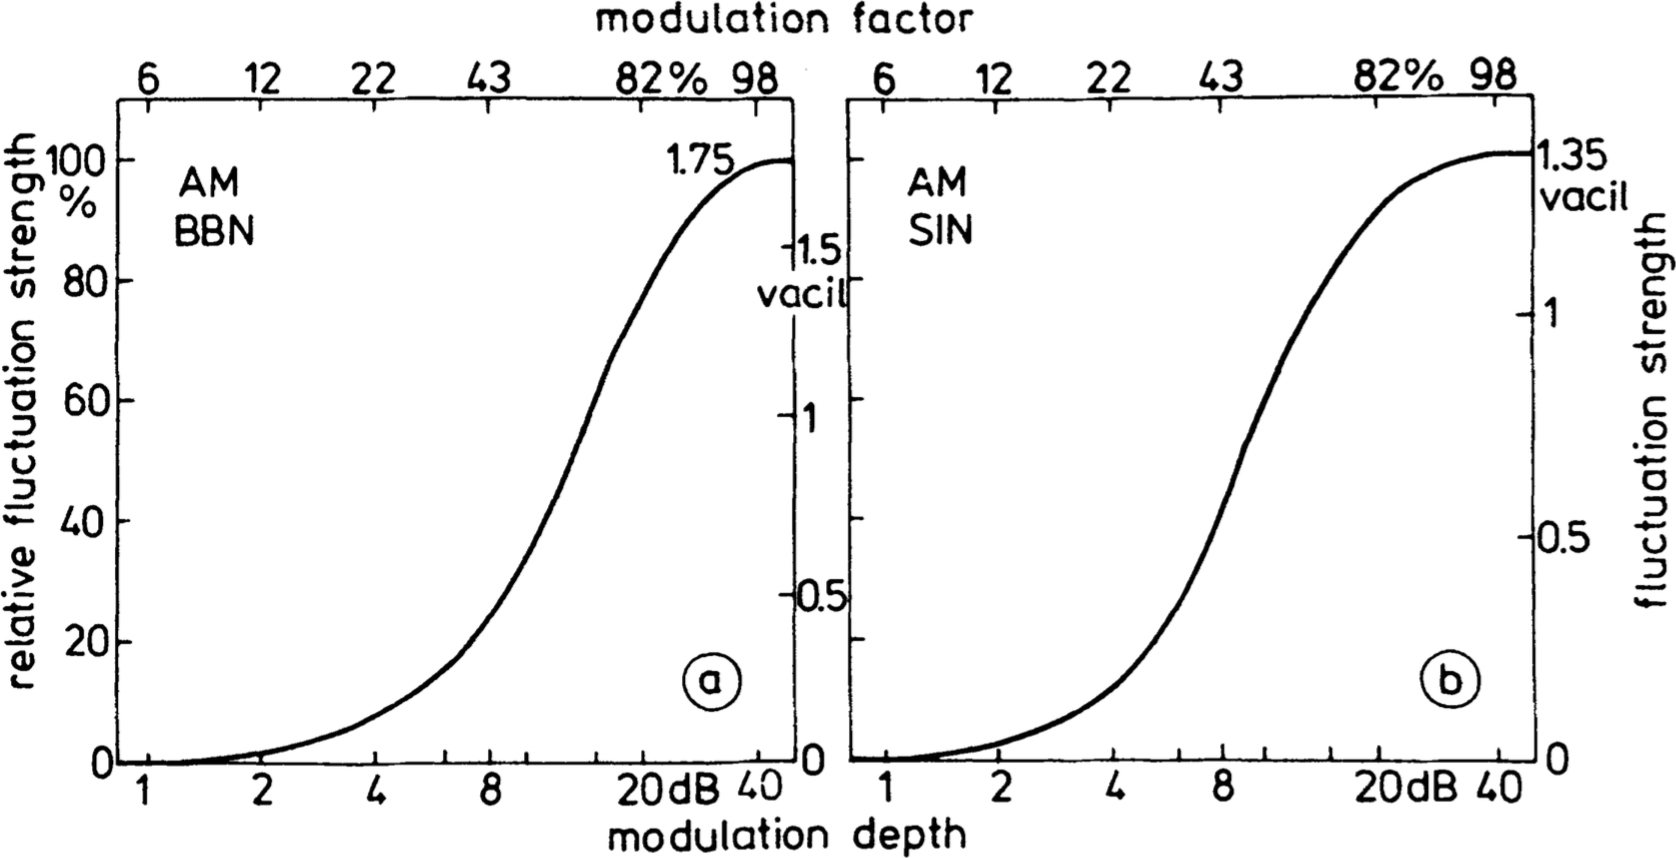
\includegraphics[height=5cm]{FluctuationStrengthVsModulationDepth}
  \caption{Fluctuation strength as a function of modulation depth for (a)
    amplitude-modulated broad-band noises of 60 dB SPL and (b)
    amplitude-modulated tones of 70 dB SPL and 1 kHz frequency; both with a
    modulation frequency of 4 Hz~\cite[pp.~249]{Fastl2007Psychoacoustics}}
\label{fig:flucstrenvsmoddep}
\end{figure}

\Cref{fig:flucstrenvscfreq} shows the relation between the center
frequency and fluctuation strength. Here a clear difference exists between the
type of modulation used. For amplitude-modulated tones there is a small
variability in the fluctuation strength, implying this a very little dependence
of the modulation frequency on fluctuation strength. For frequency-modulated
tones a clear dependence between both variables exists. For modulation
frequencies below 1 kHz the fluctuation strength is almost constant; above 1 kHz
it experiences a linear decrease until it fades away.

\begin{figure}
    \centering
    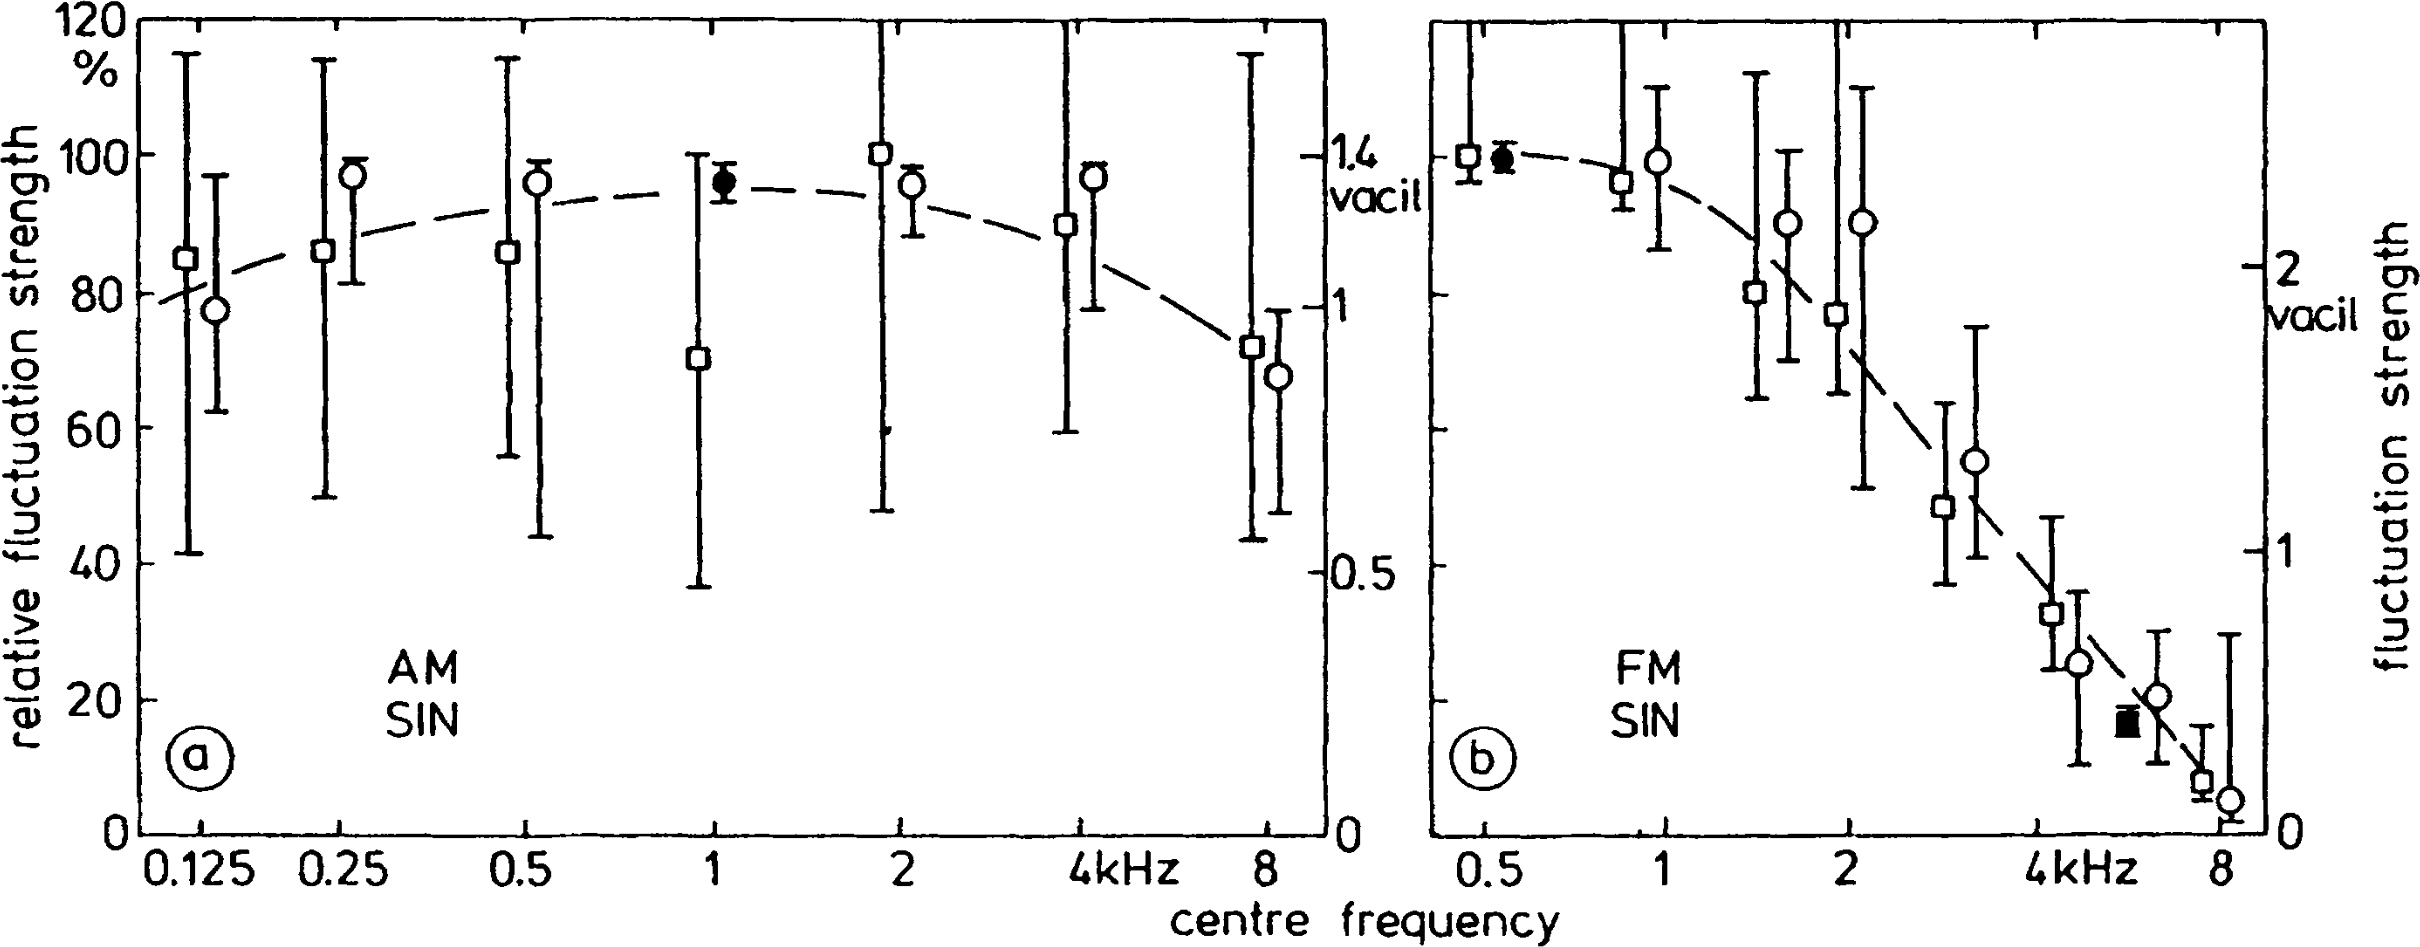
\includegraphics[height=5cm]
        {FluctuationStrengthVsCenterFrequency}
    \caption{Fluctuation strength as a function of center frequency for an
        amplitude-modulated tone of 70 dB SPL, 4 Hz modulation frequency and 40
        dB modulation depth (a), and a frequency-modulated tone with 70 dB SPL,
        4 Hz modulation frequency and $\pm200$ Hz frequency deviation
        \cite[pp. 250]{Fastl2007Psychoacoustics}}
    \label{fig:flucstrenvscfreq}
\end{figure}

To understand why this change of fluctuation strength occurs in the case of the
frequency-modulated tones, it is necessary to take into account the excitation
patterns that the modulated sounds cause regarding auditory filters. The
auditory filters are a series of overlapping bandpass filters that model the
frequency selective response of the auditory system. The excitation pattern
refers to the pattern that results as the outcome of all the precedent phases of
in the hearing process, being them the outer ear transmission, middle ear
transmission, and the auditory filters themselves.

In the case of fluctuation strength, for a 0.5 kHz tone the frequency would vary
between 300 and 700 Hz, this corresponding to a 3.5 Bark interval. For a 8 kHz
these values would be 7.8 kHz and 8.2 kHz, leading to a 0.2 Bark interval. The
proportion between these two is 17.5, which seems to be also the proportion
between the relative fluctuation strength for these two frequencies. Thus, this
leads to the idea that fluctuation strength can be explained in terms of the
excitation patterns that present themselves across the auditory filters.

Regarding fluctuation strength and frequency deviation, figure
\ref{fig:flucstrenvsfreqdev} depicts the relation between these two variables.
It can be seen that, after a frequency deviation of 20 Hz, there is a linear
increase of fluctuation strength with frequency.

\begin{figure}
  \centering
  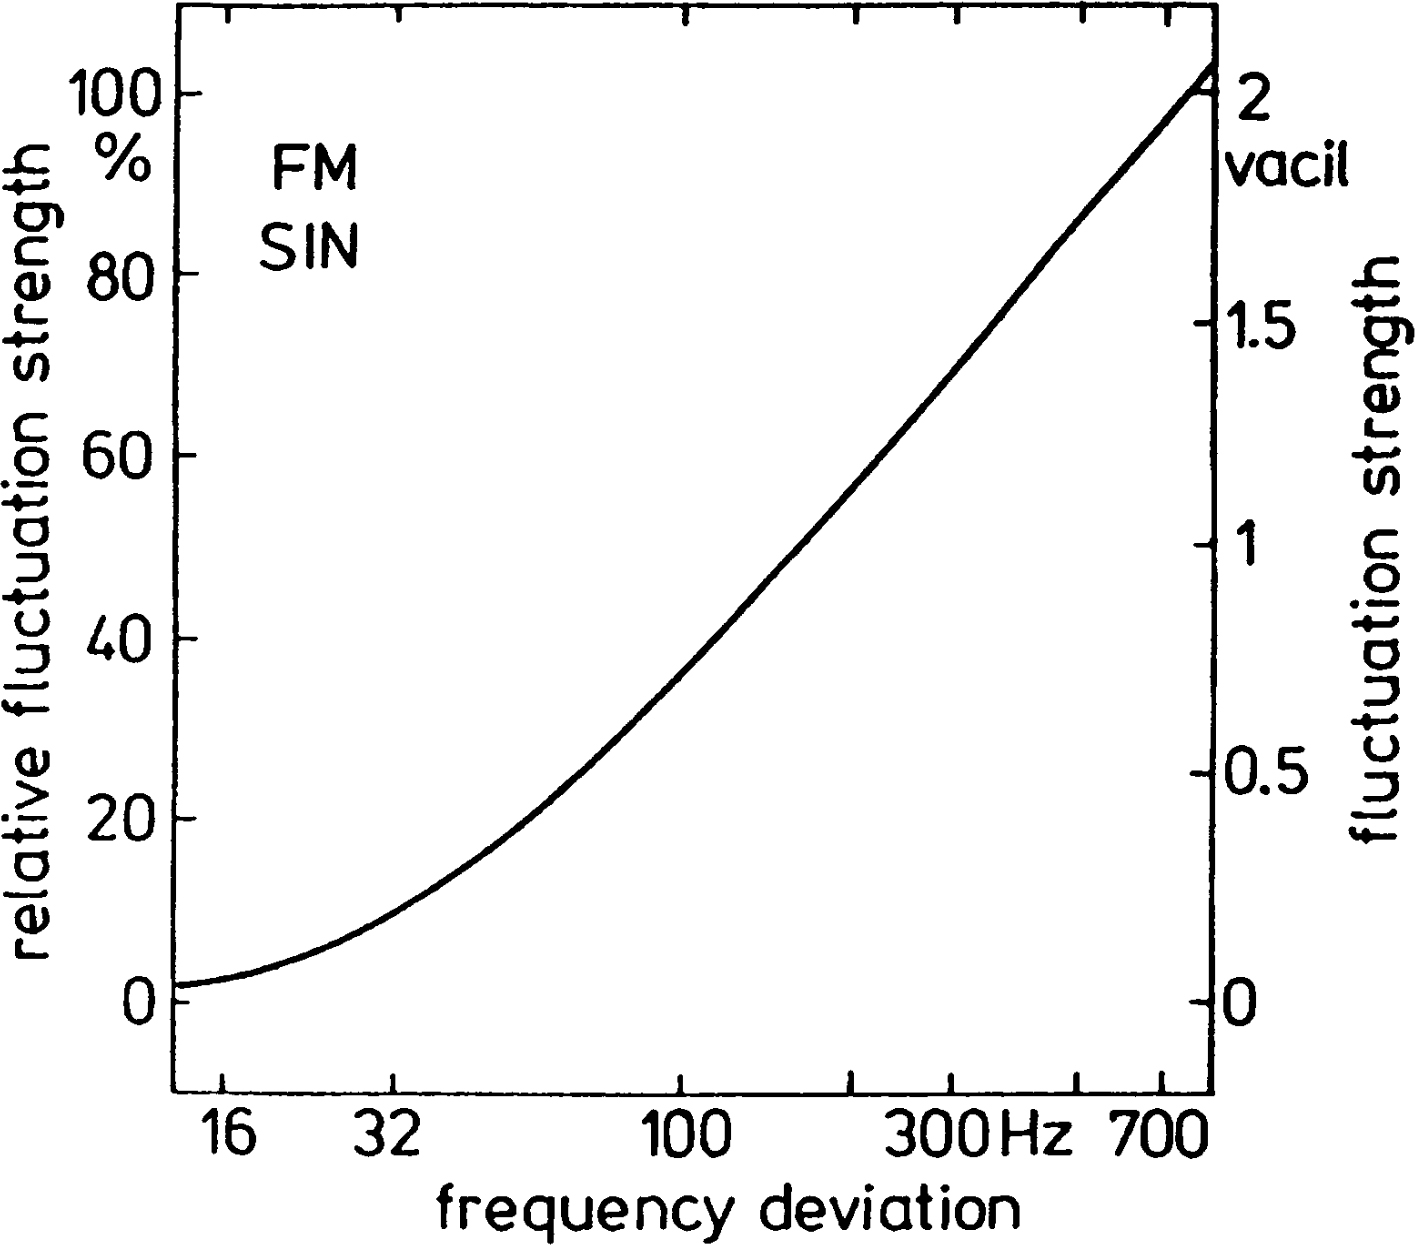
\includegraphics[height=5cm]
        {FluctuationStrengthVsFrequencyDeviation}
    \caption{Fluctuation strength as a function of frequency deviation for a
        tone with 70 dB SPL, 1.5 kHz center frequency and a modulation frequency
        of 4 Hz \cite[pp. 251]{Fastl2007Psychoacoustics}}
    \label{fig:flucstrenvsfreqdev}
\end{figure}

Another variable that affects fluctuation strength is the modulation index $h$
(also called modulation factor $m$). It is defined differently according to the
type of modulation used:
\begin{itemize}
    \item For amplitude-modulated signals is the ratio between the modulating
        signal amplitude $M$ and the carrier signal amplitude $A$,
        \begin{equation}
            h=\frac{M}{A}
        \end{equation}
    \item For frequency-modulated signals is the ratio between the maximum
        frequency deviation in the carrier signal ($\Delta f$) and the maximum
        frequency component of the modulating signal ($f_m$),
        \begin{equation}
            h=\frac{\Delta f}{f_m}
        \end{equation}
\end{itemize}

Then, regarding modulation index, it seems that a significant fluctuation
strength (10\% of the relative fluctuation strength, as defined by the authors)
is achieved with a modulation index that would correspond to about 10 times to
JND for modulation frequency. This would relate both the thresholds of
modulation frequency and fluctuation strength.

Not only modulated sounds can cause fluctuation strength, but also for non
modulated narrow-band noise. Figure \ref{fig:flucstrenvsbandwith} illustrates
this, where it can be seen that also at a 4 Hz frequency the maximum value for
fluctuation strength occurs. Regarding the SPL it behaves similarly as the other
sound sources.

\begin{figure}
    \centering
    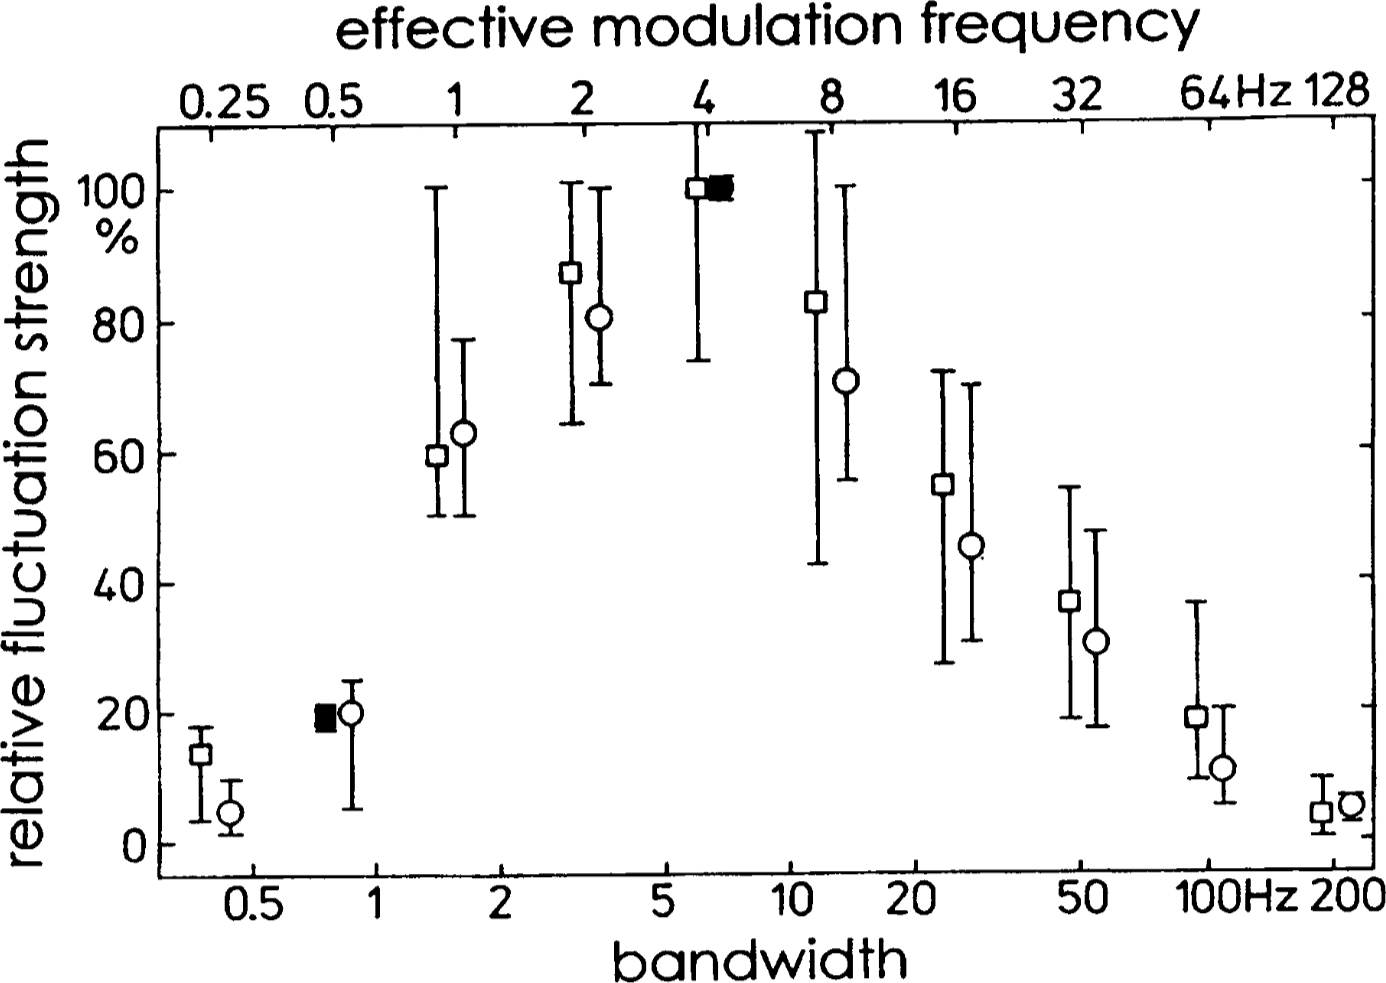
\includegraphics[height=5cm]
        {FluctuationStrengthvsBandwidth}
    \caption{Fluctuation strength as a function of bandwidth for non modulated
        narrow-band noise with 70 dB SPL and a center frequency of 1 kHz
        \cite[pp. 252]{Fastl2007Psychoacoustics}}
    \label{fig:flucstrenvsbandwith}
\end{figure}

Figure \ref{fig:flucstrensnds} compares the fluctuation strength of several
sounds, which physical characteristics are described in Table
\ref{tab:flucstrensnds}. The sounds that present the largest fluctuation
strength (1 and 2) can be related by the fact that they excite a large range of
frequencies taking into account the auditory filters. As so, it can be said that
fluctuation strength sums across critical bands.

\begin{figure}
    \centering
    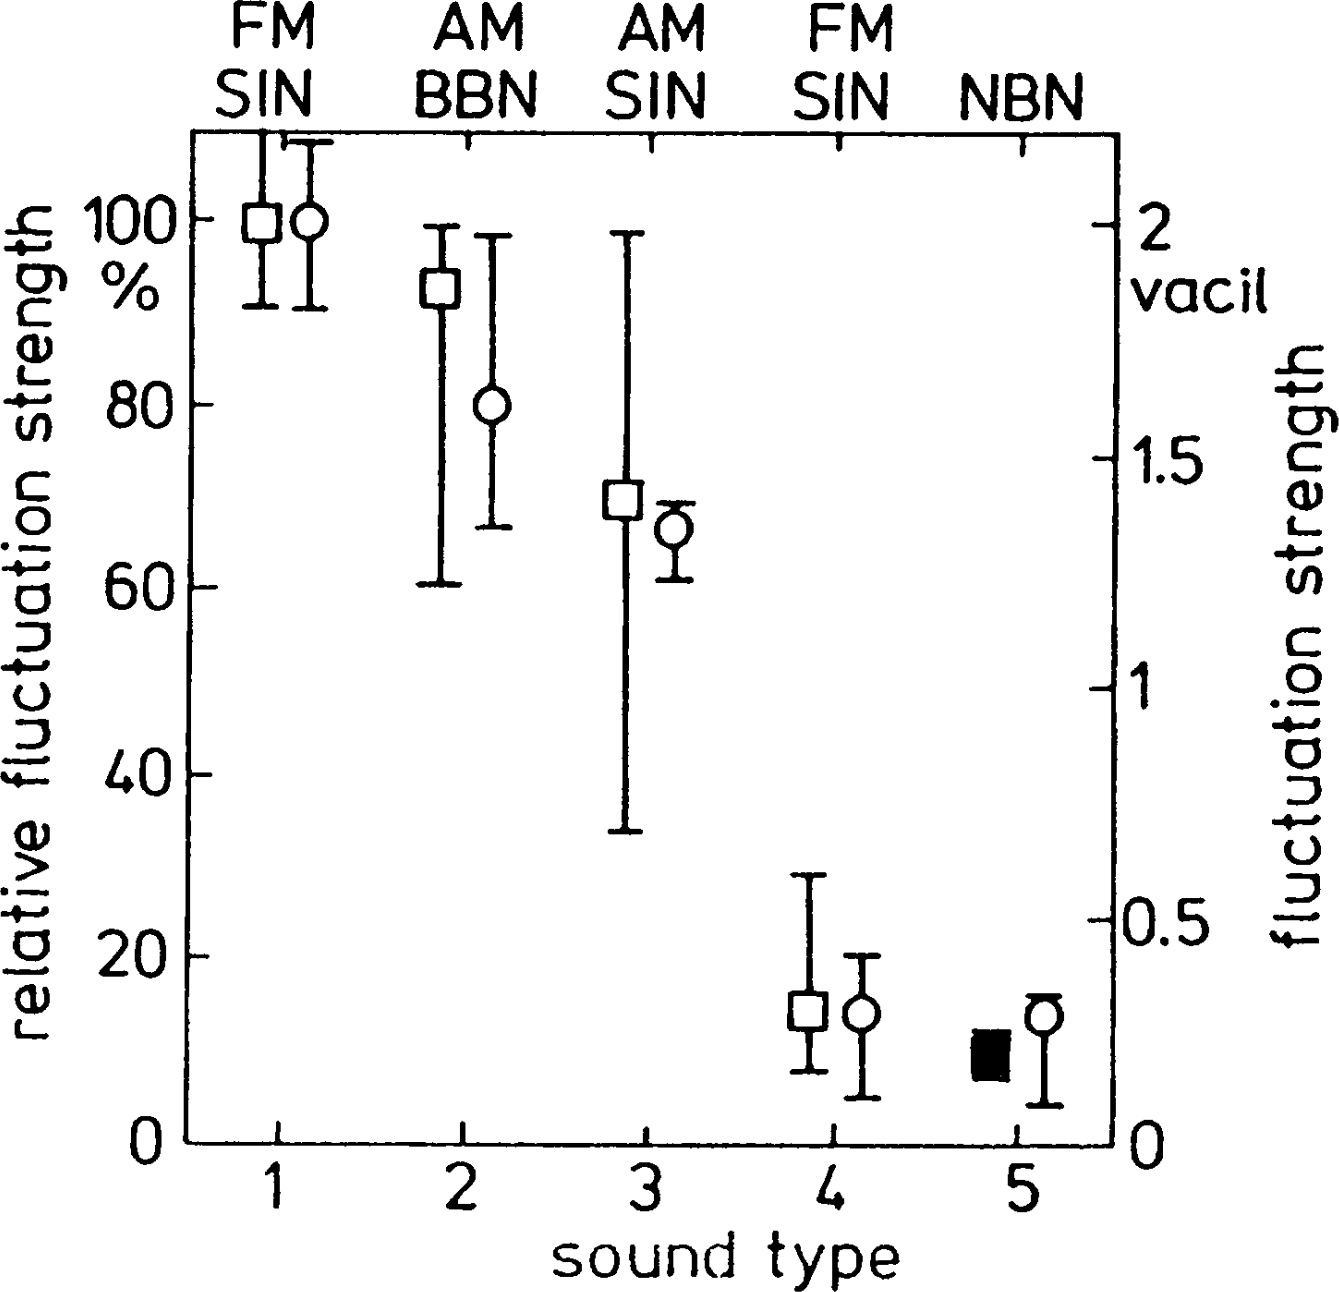
\includegraphics[height=5cm]
        {FluctuationStrengthSounds}
    \caption{Fluctuation strength of sounds 1--5 as described in Table
        \ref{tab:flucstrensnds} \cite[pp. 252]{Fastl2007Psychoacoustics}}
    \label{fig:flucstrensnds}
\end{figure}

\begin{table}
    \centering
    \begin{tabular}{ l r r r r r }
        \toprule
        Sound & 1 & 2 & 3 & 4 & 5 \\
        \midrule
        Abbreviation & FM & AM & AM & FM & \\
        & SIN & BBN & SIN & SIN & NBN \\
        Frequency [Hz] & 1500 & --- & 2000 & 1500 & 1000 \\
        Level [dB] & 70 & 60 & 70 & 70 & 70 \\
        Modulation frequency [Hz] & 4 & 4 & 4 & 4 & --- \\
        Modulation depth [dB] & --- & 40 & 40 & --- & --- \\
        Frequency deviation [Hz] & 700 & --- & --- & 32 & --- \\
        Bandwidth [Hz] & --- & 16000 & --- & --- & 10 \\
        \bottomrule
    \end{tabular}
    \caption{Physical data of sounds 1--5
        \cite[pp. 253]{Fastl2007Psychoacoustics}}
    \label{tab:flucstrensnds}
\end{table}

\subsection{Model of Fluctuation Strength}

A basic model on the temporal variation of a masking pattern in shown on Figure
\ref{fig:flucstrenmodel}, where the temporal variation of the amplitude of the
masker, also called temporal masking depth, is denoted by the magnitude
$\Delta L$. The inverse of the time difference between peak corresponds to the
modulation frequency $f_{mod}$.

\begin{figure}
    \centering
    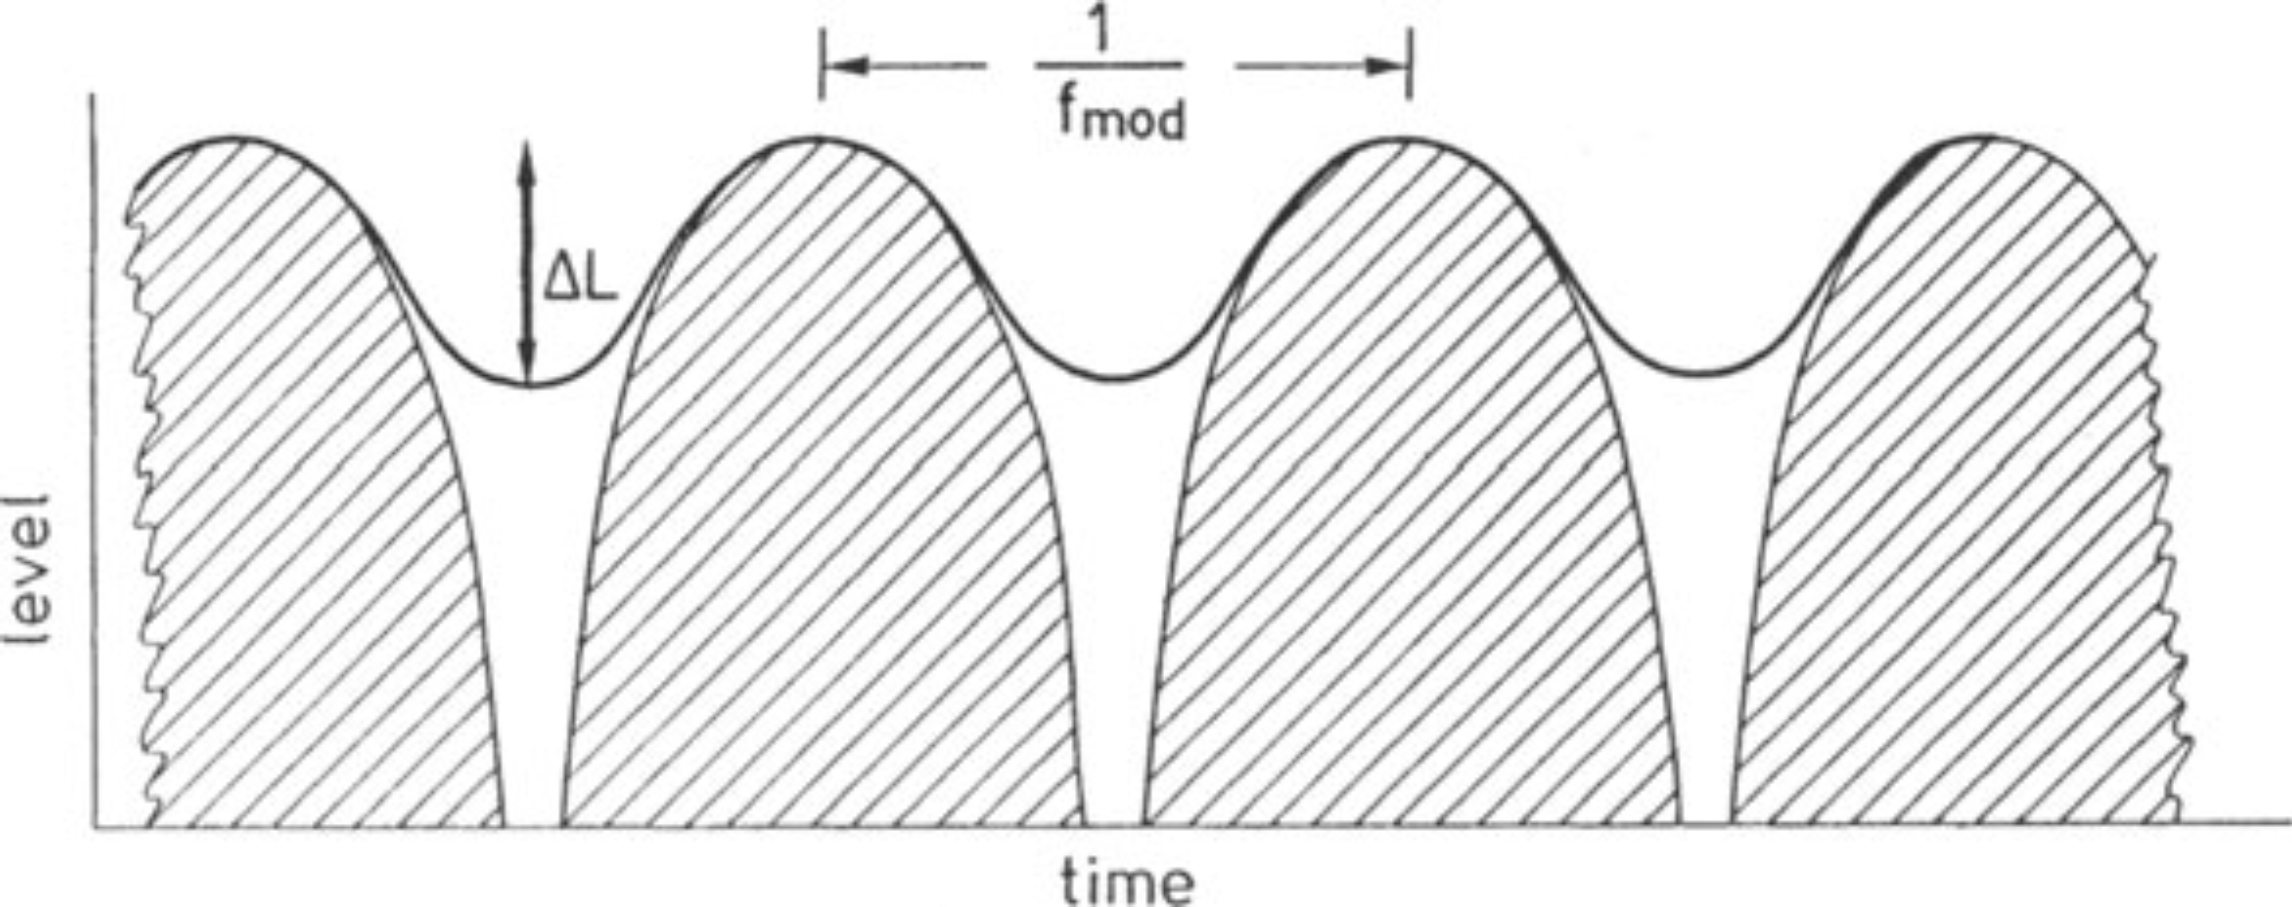
\includegraphics[height=5cm]
        {FluctuationStrengthModel}
    \caption{Model of fluctuation strength
        \cite[pp. 254]{Fastl2007Psychoacoustics}}
    \label{fig:flucstrenmodel}
\end{figure}

Equation \ref{eq:flucstrentempmaskmodfreq} shows the relationship between
fluctuation strength $F$, temporal masking depth $\Delta L$ and modulation
frequency $f_{mod}$, where the importance of the 4 Hz frequency is emphasized.

\begin{equation}
    F \sim \frac{\Delta L}{(f_{mod}/4\text{ Hz}) + (4\text{ Hz}/f_{mod})}
    \label{eq:flucstrentempmaskmodfreq}
\end{equation}

It is to note that there is dependency between the temporal masking depth
$\Delta L$ and the modulation frequency depending on the type of stimuli. In the
case of broad-band noise, temporal masking depth seems largely unaffected by
modulation frequency, whereas amplitude and frequency modulates tones these two
variable are dependent on each other, this being strongest on the frequency
modulated case. In order to address this, when modeling fluctuation strength
for these tones not a single $\Delta L$ value is taken, but instead it is
integrated across the critical-band rate scale.

Figure \ref{eq:flucstrentempmaskmodfreq} shows the resulting temporal masking
pattern for several values of modulation frequency. It can be seen that, as the
modulation frequency increases, the temporal masking depth decreases. This leads
to the idea that, although fluctuation strength presents a bandpass response
with respect to modulation frequency, the temporal masking suffers from a
low pass effect. It can be considered that the temporal masking depth decreases
linearly with modulation frequency.

\begin{figure}
    \centering
    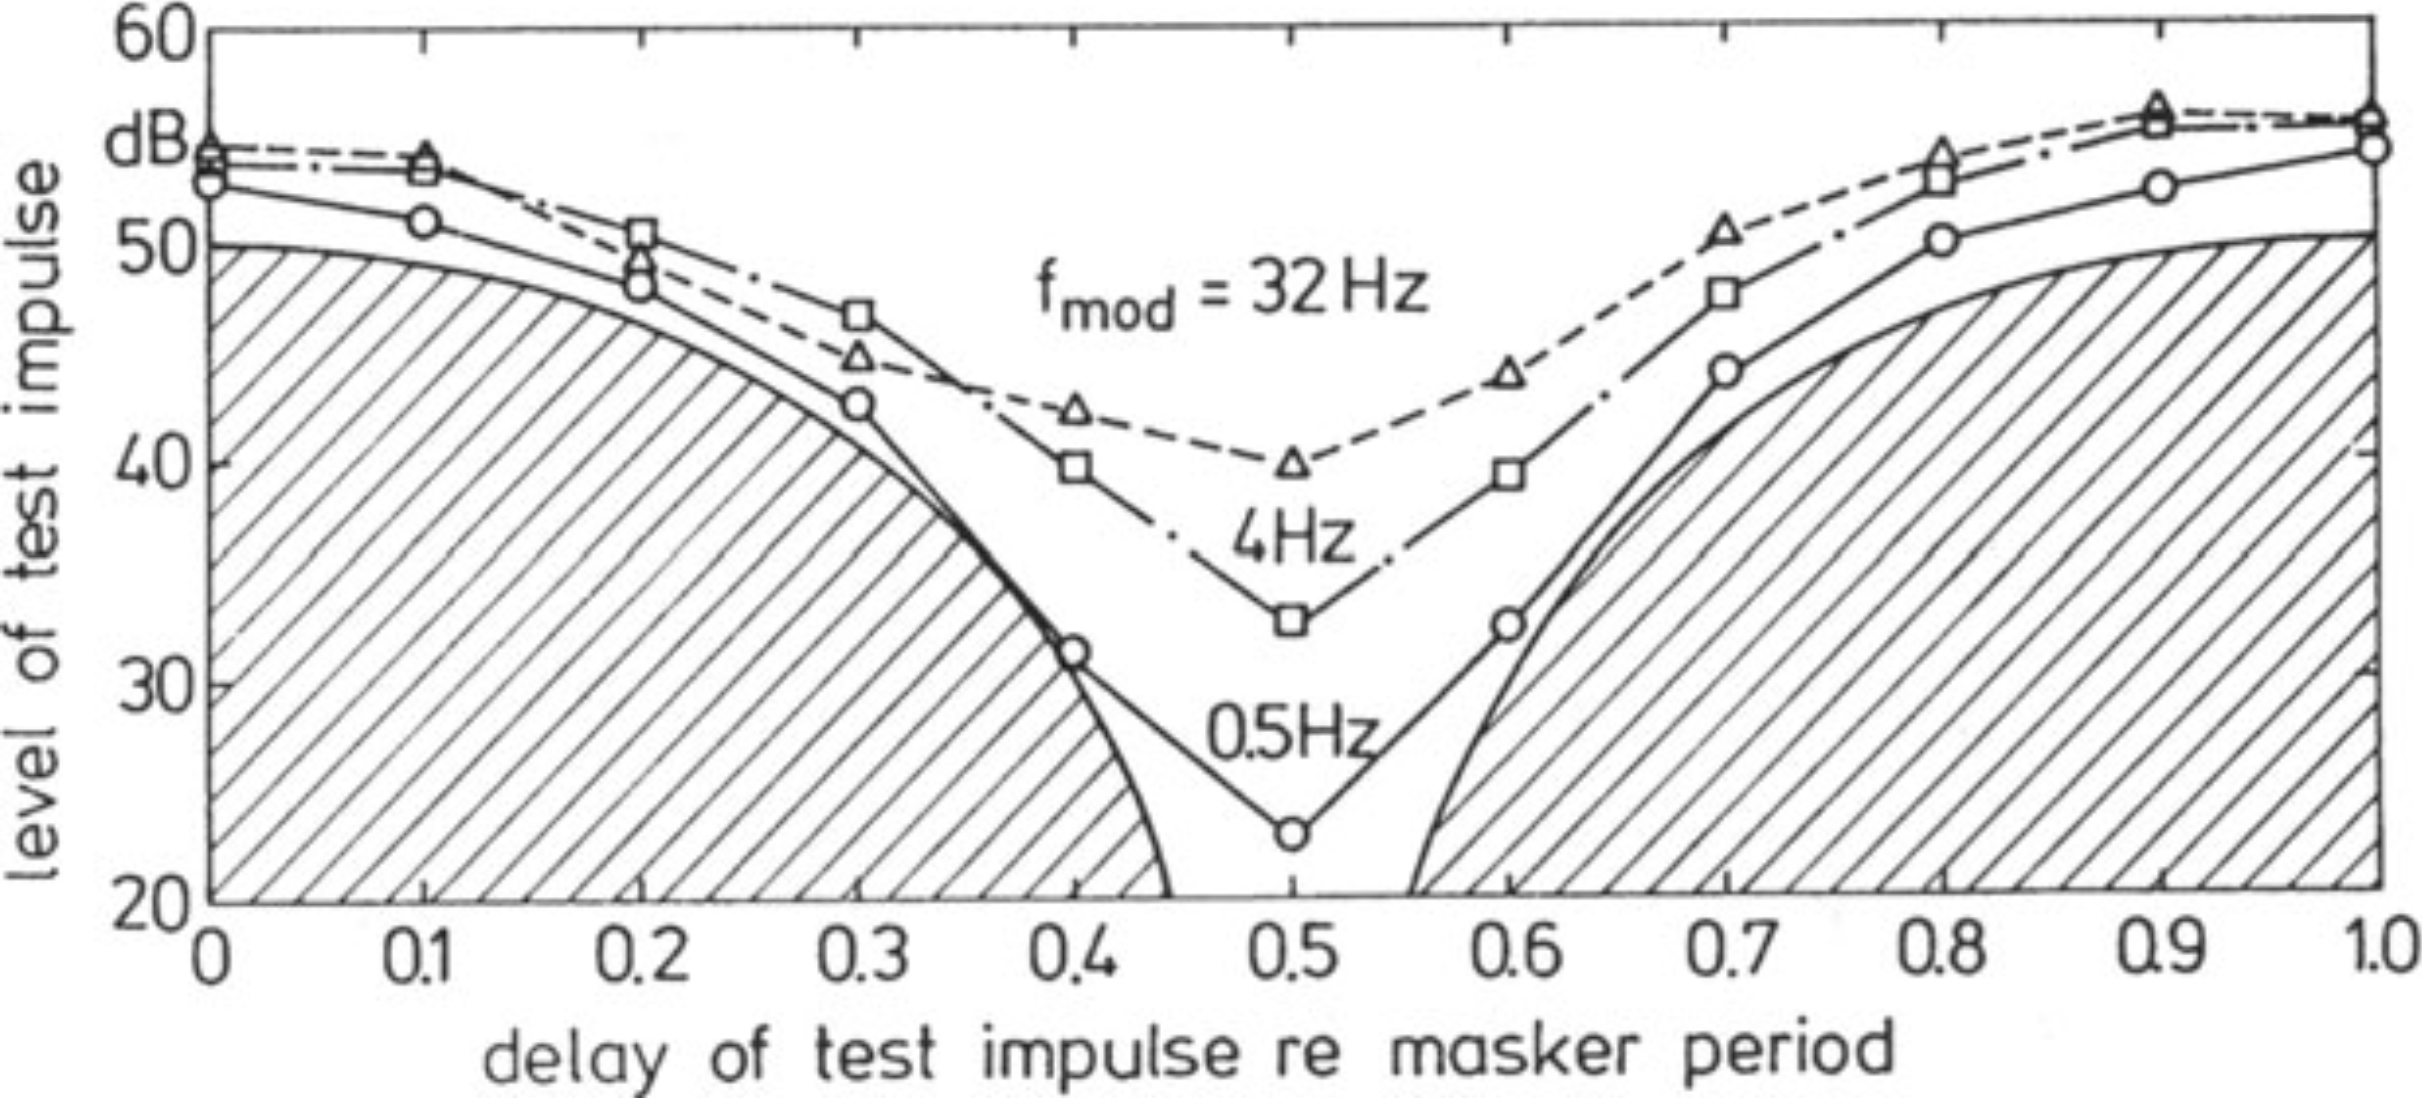
\includegraphics[height=5cm]
        {FluctuationStrengthTemporalMasking}
    \caption{Temporal masking pattern for an amplitude-modulated broad-band
        noise \cite[pp. 255]{Fastl2007Psychoacoustics}}
    \label{fig:flucstrenmasking}
\end{figure}

Taking all these into account, equation \ref{eq:flucstrenexbbn} presents an
updated model, in which $m$ is the modulation factor, and $L_{BBN}$ is the level
of broad-band noise. Similarly, equation \ref{eq:flucstrenexamfm} presents the
equivalent for the tone signals, where the temporal masking depth is integrated
across the auditory filters.

\begin{equation}
    F_{BBN} = \frac{5.8(1.25m-0.25)[0.05(L_{BBN}/\text{dB})-1]}
        {(f_{mod}/5\text{ Hz})^2+(4\text{ Hz}/f_{mod})+1.5} \text{ vacil}
    \label{eq:flucstrenexbbn}
\end{equation}

\begin{equation}
    F = \frac{0.008 \int_0^{24\text{ Bark}}(\Delta L/\text{dB Bark})\mathrm{d}z}
        {(f_{mod}/4\text{ Hz})+(4\text{ Hz}/f_{mod})} \text{ vacil}
    \label{eq:flucstrenexamfm}
\end{equation}

\end{document}
